\documentclass[tikz,border=2pt,png]{article}
\usepackage{tikz}
\usepackage{pgfplots}
\begin{document}
\title{ASSIGNMENT 05}
\author{Muneeb Ahmad Sheikh}
\date{\today}
\maketitle

\begin{itemize}
\item{\textbf{Question 2.50:}}\\

\textit{Construct a KITE EASY $AY=8cm$, $EY=4cm$ and $SY=6$:}\\


\item{\textbf{Solution:}}\\

Given,\\

$AY=8cm$, $EY=4cm$ and $SY=6$\\

Now,\\

\textit{Steps of Construction are:}\\
$

1: Draw a line AY=8cm.\\

2: Draw PQ, the perpendicular bisector of AY such that it meets AY at O.\\

3: We can't locate a point E on PQ at 4cm from Y  and A, i.e. EY=4cm=EA is not possible only when E and O coincide. In that case the  KITE doesn't exist.\\
$
\newpage
\item{\textbf{Question 2.51:}}\\

\textit{Draw a circle of diameter 6.1:}

\item{\textbf{Solution:}}\\

we're given with the diameter of circle,\\

\hspace{4 cm}$D=6.1$\\

Or, \hspace{3 cm}$radius=r=6.1/2=3.05$\\

\textit{Steps of Construction:}\\
$

1: Taking a fixed point(say O) as center.\\

2: Draw a circle of radius 3.05.\\

3: We'll get the circle of required diameter.\\
$
\newpage 
   From the construction required circle is given below:\\
    
 \begin{centre}
 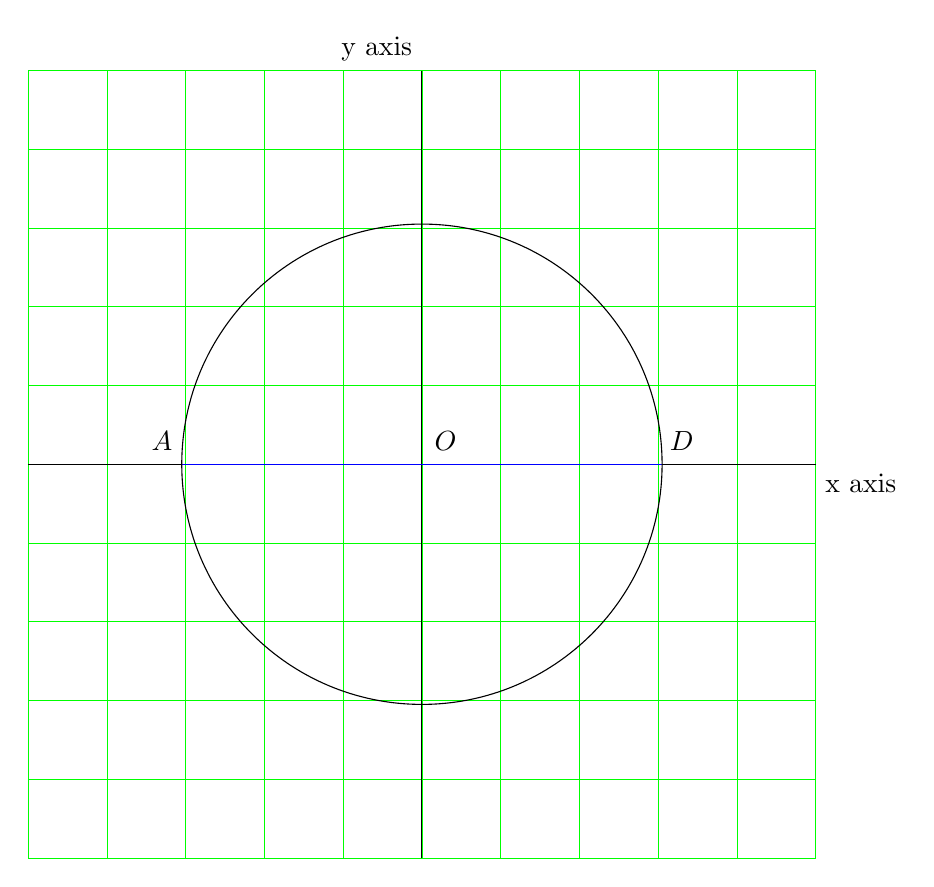
\begin{tikzpicture}
 \draw[green,very thin](-5,-5) grid (5,5);
 \draw (-5,0)--(5,0)node[anchor=north west] {x axis};
 \draw (0,-5)--(0,5)node[anchor=south east] {y axis};
 \node at (0.3,0.3){$O$};
 \draw[blue] (-3.05,0)--(3.05,0);
 \node at (-3.3,0.3){$A$};
 \node at (3.3,0.3){$D$};
 \draw (0,0) circle (3.05 cm);
 \end{tikzpicture}
 \end{centre}\\
 
\textit{$AD=6.1 cm$  is the diameter of a Circle.}

\end{itemize}
\end{document}